\documentclass[a4paper]{report}

%uncomment to see the references
%\usepackage{showkeys}
\usepackage[T2A]{fontenc}

\usepackage{algorithm}
\usepackage{algorithmic}
\usepackage[english,russian]{babel}

\usepackage[backend=biber,sorting=none,sortcites=true,bibstyle=sty/gost71,maxnames=99,citestyle=numeric-comp,babel=other]{biblatex}

\defbibenvironment{bibliography}
  {\list
     {\printfield[labelnumberwidth]{labelnumber}.}
     {\setlength{\labelwidth}{2\labelnumberwidth}%
      \setlength{\leftmargin}{\labelwidth}%
      \setlength{\labelsep}{\biblabelsep}%
      \addtolength{\leftmargin}{\labelsep}%
      \setlength{\itemsep}{\bibitemsep}%
      \setlength{\parsep}{\bibparsep}}%
      \renewcommand*{\makelabel}[1]{\hss##1}}
  {\endlist}
  {\item}


\usepackage[utf8]{inputenc}
\usepackage{csquotes}
%\usepackage{expdlist}
%\usepackage[nottoc,notbib]{tocbibind}
\usepackage[pdftex]{graphicx}
\graphicspath{{pic/}}
\usepackage{amsmath}
\usepackage{amssymb}
\usepackage{amsthm}
\usepackage{amsfonts}
\usepackage{amsxtra}
\usepackage{sty/dbl12}
%\usepackage{srcltx}
\usepackage{epsfig}
%\usepackage{verbatim}
\usepackage{sty/rac}
\usepackage{listings}
\usepackage[singlelinecheck=false]{caption}

\usepackage{xcolor, colortbl}
\definecolor{light-gray}{RGB}{230,230,230}

%%%%%%%%%%%%%%%%%%%%%%%%%%%%%%%%%%%%%%%%%%%%%%%%%%%%%%%%%%%%%%%%%%%%%%%%%%%%%%

\captionsetup[figure]{justification=centering,   position=bottom, skip=0pt}
\captionsetup[table] {justification=raggedright, position=top,    skip=0pt}

% Redefine margins and other page formatting

\setlength{\oddsidemargin}{0.5in}

% Various theorem environments. All of the following have the same numbering
% system as theorem.

\theoremstyle{plain}
\newtheorem{theorem}{Теорема}
\newtheorem{prop}[theorem]{Утверждение}
\newtheorem{corollary}[theorem]{Следствие}
\newtheorem{lemma}[theorem]{Лемма}
\newtheorem{question}[theorem]{Вопрос}
\newtheorem{conjecture}[theorem]{Гипотеза}
\newtheorem{assumption}[theorem]{Предположение}

\theoremstyle{definition}
\newtheorem{definition}[theorem]{Определение}
\newtheorem{notation}[theorem]{Обозначение}
\newtheorem{condition}[theorem]{Условие}
\newtheorem{example}[theorem]{Пример}
%\newtheorem{algorithm}[theorem]{Алгоритм}
\floatname{algorithm}{Листинг}
\renewcommand{\algorithmicrequire}{\textbf{Вход:}}

%\newtheorem{introduction}[theorem]{Introduction}

\renewcommand{\proof}{\\\textbf{Доказательство.}~}

\def\startprog{\begin{lstlisting}[language=Java,basicstyle=\normalsize\ttfamily]}

%\theoremstyle{remark}
%\newtheorem{remark}[theorem]{Remark}
%\include{header}
%%%%%%%%%%%%%%%%%%%%%%%%%%%%%%%%%%%%%%%%%%%%%%%%%%%%%%%%%%%%%%%%%%%%%%%%%%%%%%%

\numberwithin{theorem}{chapter}        % Numbers theorems "x.y" where x
                                        % is the section number, y is the
                                        % theorem number

%\renewcommand{\thetheorem}{\arabic{chapter}.\arabic{theorem}}

%\makeatletter                          % This sequence of commands will
%\let\c@equation\c@theorem              % incorporate equation numbering
%\makeatother                           % into the theorem numbering scheme

%\renewcommand{\theenumi}{(\roman{enumi})}

%%%%%%%%%%%%%%%%%%%%%%%%%%%%%%%%%%%%%%%%%%%%%%%%%%%%%%%%%%%%%%%%%%%%%%%%%%%%%%

\binoppenalty=10000
\relpenalty=10000

\addbibresource{thesis.bib}

\begin{document}

% Begin the front matter as required by Rackham dissertation guidelines
\initializefrontsections

\pagestyle{title}

\begin{center}
Санкт-Петербургский национальный исследовательский университет \\ информационных технологий, механики и оптики

\vspace{2cm}

Факультет информационных технологий и программирования

Кафедра компьютерных технологий

\vspace{3cm}

{\Large Афанасьева Арина Сергеевна}

\vspace{2cm}

\vbox{\LARGE\bfseries
Выбор вспомогательных оптимизируемых величин для ускорения процесса оптимизации\\ с помощью машинного обучения
}

\vspace{4cm}

{\Large Научный руководитель: ассистент кафедры КТ М.~B.~Буздалов}

\vspace{6cm}

Санкт-Петербург\\ 2012
\end{center}

\newpage

\setcounter{page}{3}
\pagestyle{plain}

\tableofcontents
%\listoffigures

% Chapters
\startthechapters
\startprefacepage

Задача построения карты глубины по нескольким изображениям является основополагающей в области стереозрения. Восстановление 3D$-$модели во всех вариациях задач сводится к восстановлению карты глубины. Эта фундаментальная проблема была и остается предметом множественных исследований и споров. На данный момент существует большое количество подходов к решению, но все делятся на две категории: локальные и глобальные. Локальные алгоритмы отличаются меньшей точностью и большей производительностью, в то время как глобальные дают очень хорошие результаты, но неприемлемы для приложений реального времени. Алгоритм Semi-Global matching, разработанный Хейко Хиршмюллером, позволяет получить приемлемый результат по качеству и времени. Тем не менее, алгоритм SGM не позволяет обрабатывать изображения высокого разрешения в реальном времени.

В данной работе исследуется возможность ускорения Semi$-$Global matching с помощью использования приблизительной карты глубины. Данный подход позволит уменьшить время работы алгоритма Semi-Global Matching за счёт уменьшения возможных значений диспаратности в каждой точке. В дальнейшем мы сможем использовать комбинацию быстрого локального алгоритма и разработанного метода, такая комбинация сравнима по качеству со стандартным алгоритмом SGM, но превосходит по производительности.
\chapter{���������� ���������� ������ �� ������ �������� ���������}
\label{chapter_owerview}

� ���� ����� ���������� �������� ������� ���������� ���������� ������ �� ����
�������� ���������. 

� ������� ~\ref{semantics} ������� ��������� 
���������, ������������ ��� ���������� ���������� ������. 

� �������� ~\ref{codegen} � ~\ref{patternOwerview} ������� ������� ���������� 
�������� ��� ���������� ������. ��� ������� ��������� �� ��� ������: 
\begin{itemize}
\item ��������� ��� ��������� ����;
\item �������� ��������������.
\end{itemize}

\section{��������� �������� ���������}
\label{semantics}

��������� --- �������� ����� ������ �����. ��� ��� ����� ����� ��� �����,
������������ ���������. ������, �� ���������� ��������, ���� \emph{UML} �� �������������
���������� ������� � ������� �������� ��������� �������� ���������~\cite{UMLBOOK,UMLBOOK2}.
���������� ������������ ���������
�������� � ����, ��� ������ ���������� ����� � ��� �� ������ ����� ��������
��-�������. 

��������, � ������~\cite{CraneD05} �������� ������ ��������� ���������, ������� ����������������
��-������� ��� ������������� ��������� ��������. 

���������� ��������� ����������� ��������� ��������, 
������������ ��� ���������� ���������� ������.

\subsection{��������� SWITCH-����������}
\label{switch-semantics}
SWITCH-���������� --- ��� ����������� ���������� �������������� � ���������������� ����� 
����������� ����������~\cite{SWITCH}, �������� ���� � ������� �������� 
�� �������� ��������, ��� ����� �������� ��������� ���������. ��� �����
������� ���� ���������� ������ ���������� ���� ������ ����������
���������, ��� � ���� ������� � ������~\cite{SWITCH}. ������ ��������� 
���������� ��������� ����������� ���������� ����� ��������� � ���������.
��� ���������� ������� ��������������� ���� ��� �������� ������ ����������� ����������. 

� ���������� SWITCH-���������� ����� ����������� ��� ���������� ������������� ��������. 
�� �� ���� ���������� � ����������� ����� ���� ���� ������� ����� 100 ��������~\cite{is.ifmo.ru}.

������, ����� ���������, ������������ � SWITCH-����������, �������� �� ��������������� �������� �
�������� ���������� ���������. ��������� SWITCH-���������� ����������� � 
�������~\ref{switch-technology}.

\subsection{��������� \emph{Statemate} � \emph{Rhapsody}}
���������� ���������, ������������ � �������� \emph{I-Logix Statemate}~\cite{StatemateSite}. 
��� �������� ���� ������� ���������� ��� ���������� ���������� ������, ���������
������� ������� ���������� ���������. ������� � ���������, ������������ � ���~\cite{harel90statemate}, 
����� �������� �� ���������� ���������. �������� ����������� ���� ���������
�������� ������������ ������ � ������ ��������. ��-�� ����� �����������, ������������
��� �������� ��� ���������� ���� �� ����� ����� �����, ��� ����� ���� ����� ���������
�� ���������. ����� ����, ��� ��������� ������������ ���������. ��������,
� ��������� ������ � �� �������� ���������� ��������, ������� ������ ����������� 
�� ������� �����.

���������, ������������ � ��������� \emph{I-Logix Rhapsody}~\cite{HarelKugler04,RhapsodySite} ��������� �� ����
��������� \emph{Statemate}. � ��� ���� ���������� ��������� ���������� \emph{Statemate}, ��������,
���������� � ������� ������� ���������� ��������. ������, �������� ��������� � ��������� ��������, 
���-����, ��������.

����� ��������������, �������, ��� ��������� \emph{Statemate} � \emph{Rhapsody} �������� �������������
����������, ������� �� ������ �������� ����, �� ���� � ����������� ����� �� �������������
� ��������� �������. ��� ����������� ���������� ��������� ���� �� �������.




\section{�������� ��������� ����}
\label{codegen}
� ��������� ����� ��������� ���������� ����� ������� ��� ������ � ����������� \emph{UML}. 
�� ������ �� ��� ���������� ����������� ��������������� ���������� ���� ��������� �� 
\emph{UML}-���������� �������. 

������ ��������, ����������� ������������ ��� �� ���������� ���������, �������� ����.
������� ��� ������� � ����������� ������������ ��������� (��. ������~\ref{semantics}),
������� --- � ������������ �����������, ������������ ��� ���������� ����� ��������.

���������� ��������� �� ����� �������.

\subsection{\emph{Statemate} � \emph{Rhapsody}}
� ���������, ��� ��� ����������, ��������� \emph{I-Logic Statemate}~\cite{StatemateSite} � 
\emph{I-Logic Rhapsody}~\cite{RhapsodySite} �������� ������������� ����������, ��� 
�� ��������� �� �������. ��� ���� �������, ��� ������������, � ��� ����� ������������ ��
���� ��������� --- ������������ ���������~\cite{harel90statemate,HarelKugler04,RhapsodySite}.

\subsection{SWITCH-����������}
\label{switch-technology}

����� ������� ����� ����� � �����������. ���������� ��������� �������
�� $1$ �� $n$ � ����� ������� � ��������� ���������� \t{currentState} ����� �������� ���������. 
������, ���� ��������� ��������� ��������� �������� � ����������� �� �������� ���������, 
������� ����������� \tb{switch} (��� ��������� \tb{if}), ������� � ����������� �� �������� 
���������� \t{currentState} ����� ��������� ������ ������� ����.

����� ������ ������ � ���������� ������, ����������� ���������������� ��������� �
������������ \emph{UML}~\cite{FAULER,XUML}. 

���������� �������� ���� ����� ������� � SWITCH-����������~\cite{SWITCH}, � ������� 
��� ���� ������� � �������~\ref{switch-semantics}. ���������� �������� ��� ���������
���� � ����� SWITCH-����������, �������� \emph{Visio2Switch}~\cite{VisioToSwitchSite}. 

�������, ��� ������, ������������ � SWITCH-����������, �������� ������ 
��� ���������� ��������� ���������. ����� ���������, ����������� � ���� ���������� 
������������ ����� ��� ����������� �������� �������� ���������~\cite{SAMEK}, ���� 
�������� �� ����������� ������������� ��������� � ��������� ���������.

\subsection{\emph{UniMod}}
\emph{UniMod}~\cite{UniModSite} --- ��� ������ � ����� ���������� \emph{Eclipse}~\cite{EclipseSite}, 
����������� �������� ������ ������ � ���� ��������� ��������� \emph{UML}. ��� ���� �� ������������
��� �������� ���� SWITCH-����������. ����� �������, \emph{UniMod} ���������� SWITCH-����������
� ��������-���������������� ���������������� � \emph{UML}. 
\emph{UniMod} ��������� �� ������ ������������ ���, �� � ���������������� ����������� ������.

� ���������, \emph{UniMod} �� ����� ������������ ��� ����������� �������� ��������� \emph{UML}.


\section{�������� ��������������}
\label{patternOwerview}

���������� ��������� ��������� ��������������, ��������������� ��� ����������
���������, ������������� � ����������� �� ���������~\cite{GAMMA,ADAMCZYK}.
� ���� ������� ����������� ��������� �� ���.
                         
\subsection{������� \emph{State}}
������� \emph{State}, ��������� � ������~\cite{GAMMA} �������� �����
������ � ���������, ������ �� ������������ ��� ���������� ������� �����������
�������� ���������, ��������, ��������� ���������. ���������� ��������� ��� ����������~\cite{ADAMCZYK}, 
������ �� ���� �� ��� �� �������� ��� ���������� ���������� �������� ���������,
���������� ���������� ���������.

\subsection{������� \emph{State Machine}}
������� \emph{State Machine}, ��������� � ������~\cite{StateMachinePattern} 
��������� ����������� �������� \emph{State}, ������ � ������������ ����� �� ��� ��
�� ������������ ��� ���������� ������� ������, �������� ���������� ���������. 


\chapter{Постановка задачи и описание метода ее решения} 
\label{chapter2}

В данной главе обосновывается необходимость улучшения существующих подходов, описывается новый метод.

\section{Задача}
SGM является оптимальным компромиссом качества и скорости по построению карт глубин на текущий момент. Для выполнения всех шагов алгоритма Semi-Global matching требуется $ O ( W \cdot H \cdot D) $ времени и $ O ( W \cdot H \cdot  D) $ памяти, где $W$ - ширина изображения, $H$ - высота изображения, $D$ - максимальная диспаратность. Ввиду того, что $D$ зависит от размера изображения, мы получаем нелинейное возрастание времени работы алгоритма от размера изображения. Несмотря на огромную разницу в производительности относительно глобальных алгоритмов, время работы SGM на больших изображениях слишком велико и не сопоставимо со временем работы локальных алгоритмов. Качество, полученных результатов, близко к качеству глобальных алгоритмов. Поэтому попробуем изменить метод SGM для повышения скорости работы без потери качества.


\section{Метрика качества карты стереоглубины}

Качество любых алгоритмов построения карт глубин измеряется с помощью специальных пар картинок, для которых вручную созданы карты. Алгоритму подается такая пара изображений, затем по полученной с помощью него карте делается сравнение с эталонной.  Для разных задач требуется разная точность диспаратностей, поэтому при измерении качества диспаратность пикселя считается верной, если соответствующий пиксель на эталоне отличается от текущего не более, чем на определенную велечину. 

Такая метрика характеризует качество алгоритма для только определенной погрешности, поэтому алгоритмы могут давать хорошие результаты с большой погрешностью и плохие с маленькой. 

В данной работе для измерения качества использовался сервис ~\cite{middlebury} на основе множества пар изображений с картами глубин для подсчёта качества.

\section{Метод с использованием приближенных вычислений карты глубины.}

Предлагаемый метод получает на вход пару изображений, карту глубины с большой погрешностью и возвращает карту глубины с меньшей. Приближенную карту глубины мы можем посчитать с помощью быстрого, например локального, алгоритма, который строит карту с хорошим качеством при большой погрешности. 

Стандартный Semi-Global Matching, как отмечалось в разделе \ref{sgm}, состоит из вычисления попиксельной стоимости, суммирования попиксельной стоимости и вычисления карт диспартности. Чтобы улучшить асимптотическую сложность всего алгоритма, понадобится модифицировать каждый этап стандартного алгоритма.

\subsection{Оптимизация вычисления попиксельной стоимости.}
В стандартной реализации Semi-Global Matching в препроцессинге производится расчет попиксельных стоимостей для каждого пикселя по всем диспаратностям за $O ( W \cdot H \cdot D)$. В моей работе было проверено три способа вычисления: подсчет всех стоимостей, вычисление без препроцессинга во время исполнения программы, подсчет стоимостей для каждого пикселя только для допустимых диспаратностей $[min, max]$, где $min$ и $max$  минимальное и максимальное значения возможной диспаратности в данном пикселе на основе приближенного вычисления.

Изменения на данном шагу алгоритма позволили уменьшить потребляюмую оперативную память и время выполнения, так как при использовании приближенной карты глубины мы пользуемся только частью предпосчитанной информации с помощью базового метода.

\subsection{Оптимизация суммирования попиксельной стоимости}
Шаг суммирования попиксельной стоимости реализован для поиска оптимальной конфигурации на основе только допустимых значений диспаратности.

Для некоторых точек алгоритм, используемый для поиска приближенной карты глубины, может не найти точки для сопоставления, либо выдавать низкий коэффициент доверия, такой алгоритм, например, представлен в работе~\cite{esgm}. Также такие точки могут быть найдены с помощью дополнительных эвристик после построения карты. Чтобы оставить возможность находить верное сопоставление было предложено два подхода по присвоению допустимых значений:
\begin{itemize}
\item $d(x,y) = [0; max\_disparity]$
\item $d(x, y) = d(x - 1, y)$
\end{itemize}

Для точек, где значения глубины являются достоверными по версии алгоритма, значение интервала допустимых диспаратностей указано в формуле~\ref{d_int}, где $error$ - допустимая погрешность в приближении, $width$ - ширина изображения, $d\_est(x,y)$ -  предположительная диспаратность в точке $(x,y)$, $d(x,y)$ - интервал допустимых диспаратностей в точке $(x,y)$.

\begin{equation}
\label{d_int}
d(x,y) = [ max(0,  d\_est(x,y) - error); min( width, d\_est(x,y) + error)]
\end{equation}

Алгоритм минимизации функционала с помощью динамического программирования модифицируется под обработку только допустимых диспартностей. В листинге~\ref{algo} показана реализации модификации. $[d\_min(p);  d\_max(p)]$ задают интервал допустимых значений диспаратности для точки $p$. Если для точки не существует точка, для которой эта точка следующая по направлению, то эта точка является "стартовой". Минимум из четырех стоимостей более подробно представлен на формуле~\ref{minimization2}

\begin{algorithm}[h!]
\caption{Метод минимизации функционала по одному из направлений.}
\label{algo}
\begin{algorithmic}[1]
 \STATE {Создать очередь обработки точек} $queue$
 \STATE {Добавить в очередь обработки точек все точки, которые являются "стартовыми точками" по данному направлению}
 \WHILE {(очередь не пуста)}
    \STATE {Вытащить первую точку из очереди} $p$
    \FOR{($d = d\_min(p)$ to $ d\_max(p)$)} 
	\STATE {$curr \leftarrow $ стоимость соответствия точек $(p.x, p.y)$ и $(p.x + d, p.y)$}
	\STATE {$best\_value \leftarrow $ минимум из четырех стоимостей по направлению с различными диспаратностями}
	\STATE {$l[p.x][p.y][d  - d\_min(p)] \leftarrow curr + best_value $}
    \ENDFOR
    \IF{(есть следующая точка за текущей по данному направлению)}
	\STATE {Добавить в очередь следующую точку}
   \ENDIF
  \ENDWHILE
\end{algorithmic}
\end{algorithm}

Заметим, что каждый пиксель обрабатывается один раз и для каждого пикселя проводится $(d\_max(p) - d\_min(p))$ действий, тогда количество действий, выполненных для всего изображения не будет превышать $(W \cdot H \cdot \max_{p} (d\_max(p) - d\_min(p)))$. Из полученной формулы, мы можем сделать вывод, что модифицированный алгоритм на основе второго подхода по присвоению допустимых значений имеет асимптотическую сложность $O(W \cdot H \cdot error)$ и имеет такие же затраты на память. 

Время работы первого подхода зависит от качества приближения базового алгоритма:  если для многих точек алгоритм не может найти соответствие, время выполнения модифицированного будет расти до времени SGM. В случае, если базовый алгоритм для многих точек возвращает значения глубины с большей погрешностью, чем $error$, качество результата может упасть. Поэтому очень важно выбирать входной алгоритм не только по времени быстродействия и качеству карты глубины, но и по типу ошибок алгоритма: алгоритм не нашел соответствие или вернул неверный результат.


\chapter{Демонстрация особенностей метода} 
\label{chapter4}

В данной главе экспериментальным способом на примере решения модельных задач показаны некоторые особенности разработанного метода. А именно, способность метода выбирать наиболее выгодные ФП на различных этапах оптимизации, тем самым повышая производительность ЭА, а также способность игнорировать такие ФП, применение которых приводит к ухудшению целевой ФП. Таким образом, выполняются требования, предъявляемые к методу в разд.~\ref{requirements}.

\section{Модельная задача min-max}
\label{model-problem}

	\subsection{Постановка задачи}
	Рассмотрим модельную задачу, на примере которой экспериментально проверена способность метода выбирать наиболее эффективные ФП на различных этапах оптимизации.
	Особь представлена битовой строкой длиной $n$, $x$ бит которой равны единице.
	Определим целевую ФП как
	\begin{equation}
	\label{eqn_target}
	g(x)=\left\lfloor \frac{x}{d} \right\rfloor.
	\end{equation}

	Вспомогательные функции имеют вид $h_1(x) = \min(x, p)$ и $h_2(x) = \max(x, p)$,
	где $p$ --- положительное целое число. Будем называть $p$ \emph{точкой переключения}.	
	Графики описанных функций представлены на рис.~\ref{pict:h1h2g}.

	Особенностью этой задачи является наличие точки переключения, позволяющее проверить способность метода динамически выбирать наиболее выгодную на данном этапе оптимизации функцию приспособленности. 
	Для особей,  число единиц в представлении которых меньше, чем точка переключения $p$, наиболее эффективно использовать вспомогательную функцию $h_1$ в качестве текущей. 
    Для остальных особей должна быть использована функция $h_2$. Ожидается, что в таком случае особи с более высокими значениями целевой функции $g$ будут выращены быстрее, 
    чем в случае использования самой целевой функции в качестве текущей. 
	
	\begin{figure}[h!]
		\center{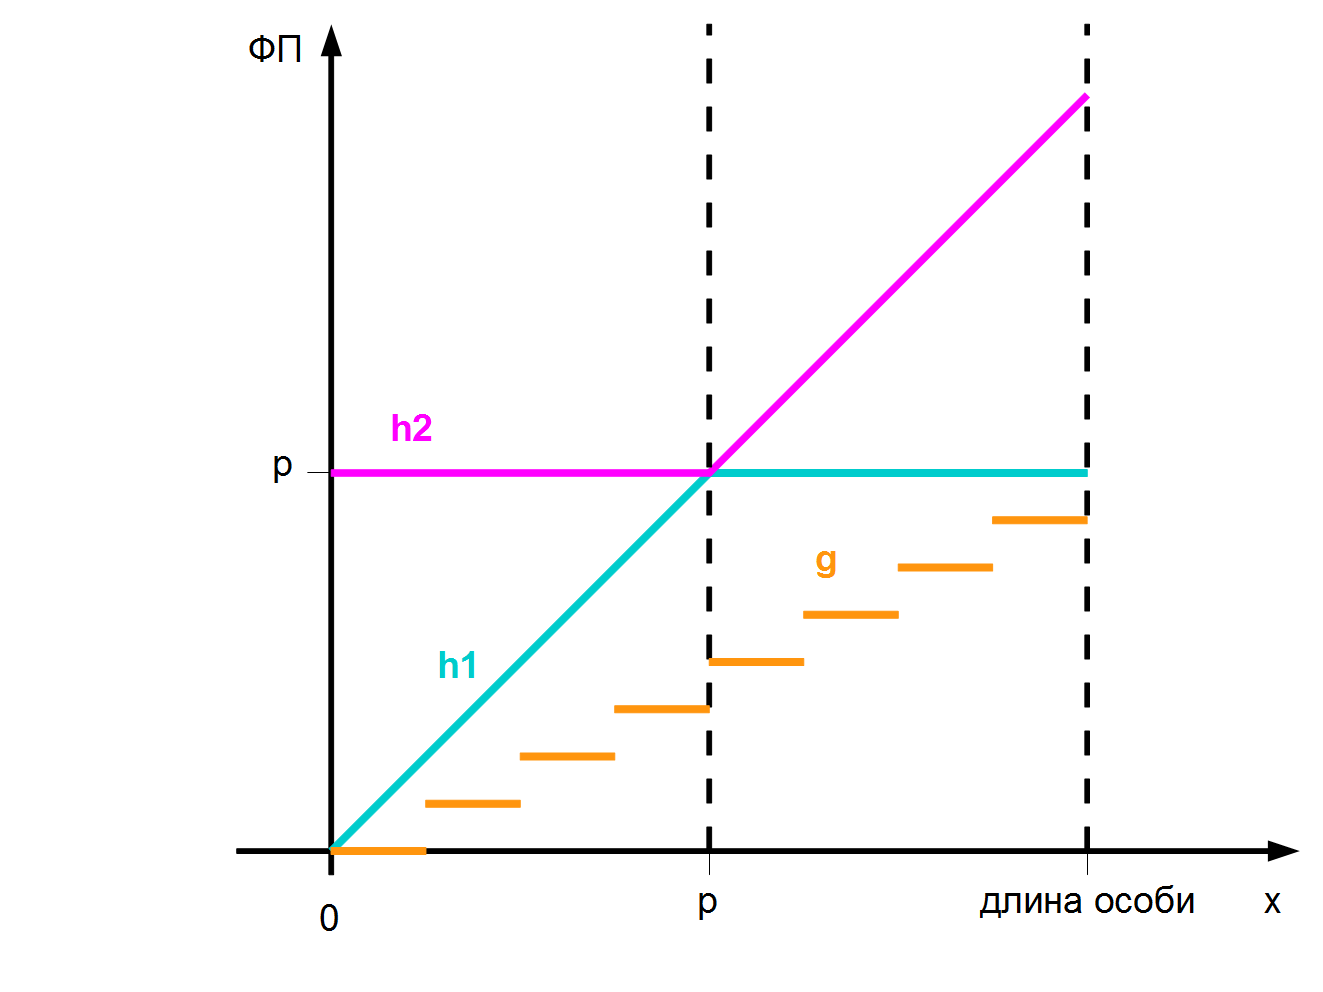
\includegraphics[width=0.6\textwidth]{h1h2g}}
		\caption{Функции приспособленности в модельной задаче}
		\label{pict:h1h2g}
	\end{figure}
		
	\subsection{Описание и результаты эксперимента}
	Был проведен ряд экспериментов, в ходе которых к решению модельной задачи применялись различные алгоритмы обучения с подкреплением, оптимизирующие генетический алгоритм (ГА). 
    Значения параметров ГА, использованные в экспериментах, представлены в табл.~\ref{experiment}. Было перебрано более тысячи различных комбинаций значений параметров обучения
    для каждого использованного алгоритма. Каждый алгоритм запускался 50 раз, и результаты, полученные с его помощью, усреднялись. Следует отметить, что наиболее выгодным значением дисконтного фактора (\ref{mark}) оказался ноль. Это указывает на то, что в данной задаче 
    информации о текущем состоянии среды достаточно для обучения и учет предыдущего опыта не требуется. 	
	
	\begin{table}[h!]
	\caption{Значения параметров, использованные в ходе эксперимента}
    \label{experiment}
	%\begin{center}
	\begin{tabular}{|l|l|} \hline
	Параметр & Значение \\ \hline
	Число запусков алгоритма & 50 \\ \hline
	Число особей в поколении & 100 \\ \hline
	Число поколений & 400 \\ \hline
	Коэффициент элитизма & 5 \\ \hline
	Вероятность кроссовера & 0.7 \\ \hline
	Вероятность мутации & 0.003 \\ \hline
	Длина особи & 400 \\ \hline
	Точка переключения & 266 \\ \hline
	Делитель $d$ & 10 \\ \hline
	\end{tabular}
	%\end{center}
	\end{table}
	
	Наилучшие результаты удалось получить, используя алгоритм обучения Q-learning c $\varepsilon$-жадной стратегией (\ref{strategy}). На рис.~\ref{pict:mm-dn-bounds} представлены графики зависимости 
    целевой ФП от номера поколения в случае использования метода, основанного на обучении, и обычного ГА. Можно видеть, что применение обучения позволяет гарантированно 
    вырастить идеальную особь менее, чем за 250 поколений. Использование обычного ГА, положенного в основу метода с обучением, не приводит к стабильному получению 
    идеальной особи в пределах использованного количества поколений, что проиллюстрировано на рис.~\ref{histogram}. Также на рис.~\ref{pict:mm-dn-bounds} находится диаграмма, отражающая число раз, когда была выбрана та или иная ФП. Отметим, что разработанный алгоритм успешно справился с выбором функций $h_1$ и $h_2$ на соответствующих этапах оптимизации.
	
	\begin{figure}[h!]
		\center{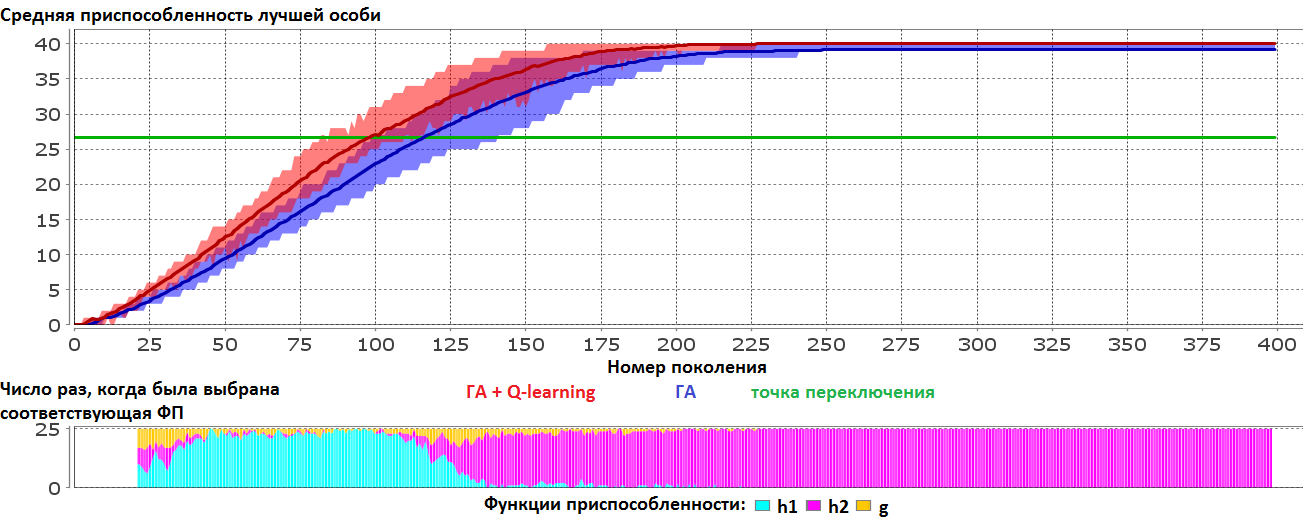
\includegraphics[width=\textwidth]{new-delayed}}
		\caption{Усредненные результаты решения модельной задачи min-max}
		\label{pict:mm-dn-bounds}
	\end{figure}
	
	\begin{figure}[h!]
		\center{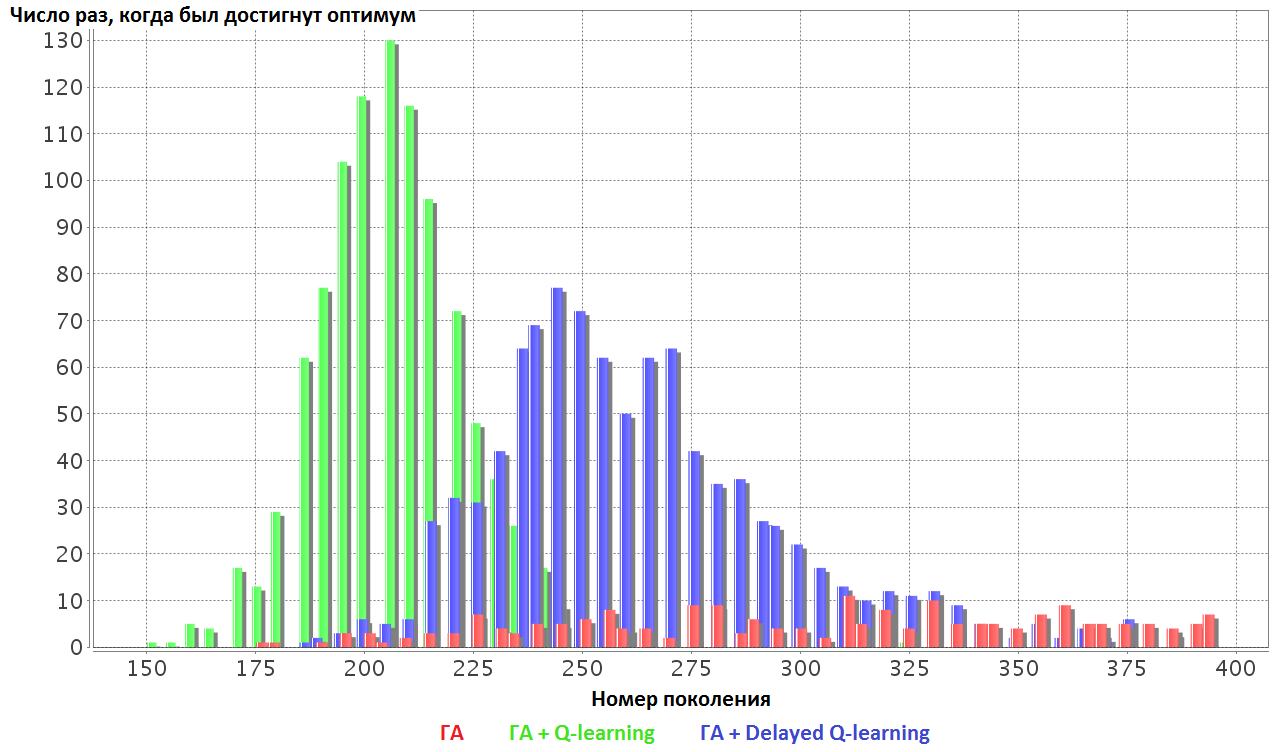
\includegraphics[width=\textwidth]{histogram1}}
		\caption{Распределение числа раз, когда было получено оптимальное решение задачи min-max, в зависимости от номера поколения}
		\label{histogram}
	\end{figure}
	
\section{Задача Royal Roads с мешающей ФП}

Рассмотрим модельную задачу, в которой оптимизация по единственной вспомогательной ФП приводит к быстрой убыли целевой. Экспериментально покажем, что определенные виды обучения способны справляться с решением такой задачи, выбирая целевую ФП. В качестве целевой ФП возьмем функцию Royal Roads \cite{mitchell-ga}. Пусть длина особи равна 64 битам. Выберем длину блока $b = 8$. Наличие очередного блока, заполненного $b$ единицами, увеличивает ФП на $b$. В качестве вспомогательной ФП будем использовать функцию, значение которой равно числу нулей, содержащихся в особи. 

В табл. \ref{royal} приведены результаты эксперимента по решению поставленной задачи. Усреднение производилось за 50 запусков каждого алгоритма. Выполнение алгоритма останавливалось при нахождении оптимума, либо при превышении максимального числа вычислений ФП, равного 500000. Число шагов в запусках, в которых не удалось получить оптимум, условно обозначено как бесконечность.

Можно видеть, что применение стратегии исследования среды по Больцману (\ref{strategy}) позволяет получить такую же производительность, что и без мешающей ФП. Использование алгоритма Delayed Q-learning, реализующего собственную стратегию исследования среды, также приводит к высоким результатам. Алгоритмы, использующие $\varepsilon$-жадную стратегию исследования среды значительно проигрывают упомянутым алгоритмам. Это можно объяснить тем, что для $\varepsilon$-жадной стратегии характерно существование постоянной вероятности $\varepsilon$, с которой выбирается случайное действие. Значит, в алгоритмах, использующих эту стратегию, всегда присутствует вероятность выбора мешающей ФП, равная $0,5\varepsilon$, что приводит к ухудшению целевой ФП. Заметим также, что установка нулевой вероятности выбора случайного действия в общем случае неэффективна (что подтверждается экспериментальными данными), так как подобный подход не позволяет агенту исследовать среду.

\begin{table}[ht]
\begin{center}
\caption{Результаты решения задачи Royal Roads} \label{royal}
\begin{tabular}{|p{4cm}|p{2cm}|p{2.5cm}|l|l|l|}
\hline
Алгоритм &\% успешных запусков & Шагов в успешных запусках (среднее) & Max шагов & Min шагов & $\sigma$\\
\hline
%\multicolumn{5}{|c|}{$(1+1)$ ЭС без мешающей ФП}\\ \hline
$(1+1)$ ЭС без мешающей ФП &100 & 6913,28 & 16033 & 2439 & 2925,07 \\ \hline
%\multicolumn{5}{|c|}{$(1+1)$ ЭС~+~Q-learning \cite{sutton} (больцмановская стратегия)}\\ \hline
ЭС~+~Q-learning \cite{sutton} (больцмановская стратегия) &100 & 6813,40 & 17252 & 2659 & 2999,60 \\ \hline
%\multicolumn{5}{|c|}{$(1+1)$ ЭС~+~Delayed \cite{delayed}}\\ \hline
$(1+1)$ ЭС~+~Delayed \cite{delayed} &88 & 8365,52 & $\infty$ & 3982 & 3216,13 \\ \hline
%\multicolumn{5}{|c|}{$(1+1)$ ЭС~+~R-learning \cite{r-learning} ($\varepsilon$-жадная стратегия)}\\ \hline
ЭС~+~R-learning \cite{r-learning} &100 & 69881,74 & 289936 & 5254 & 67990,07 \\ \hline
%\multicolumn{5}{|c|}{$(1+1)$ ЭС~+~Dyna \cite{sutton} ($\varepsilon$-жадная стратегия)}\\ \hline
ЭС~+~Dyna \cite{sutton} ($\varepsilon$-жадная стратегия) &26 & 5749,62 & $\infty$ & 2654 & 2056,78 \\ \hline
%\multicolumn{5}{|c|}{$(1+1)$ ЭС~+~Q-learning ($\varepsilon$-жадная стратегия)}\\ \hline
ЭС~+~Q-learning ($\varepsilon$-жадная стратегия) &24 & 6964,17 & $\infty$ & 3012 & 2256,70 \\ \hline
\end{tabular}
\end{center}
\end{table}

\section{Выводы по главе \protect\ref{chapter4}}
Описана модельная задача, позволяющая проверить работоспособность предлагаемого метода в случае, когда на различных этапах оптимизации выгодны различные вспомогательные ФП. 
Приведены результаты экспериментов, показывающие, что использование разработанного метода для решения описанной модельной задачи позволяет в 100\% запусков получать лучшую особь 
за конечное число поколений, в то время как с помощью ГА без обучения подобной производительности достичь не удается. В ходе эксперимента подтверждено, что разработанный метод 
динамически выбирает функцию приспособленности, наиболее выгодную на данном этапе.

Также описана задача, в которой оптимизация по вспомогательной ФП сильно ухудшает значение целевой ФП. Показано, что использование стратегии исследования среды по Больцману, а также алгоритма Delayed Q-learning, обладающего собственной стратегией исследования среды, позволяет получать такую же производительность, как в случае отсутствия мешающей ФП. Иначе говоря, обучение способно успешно игнорировать неэффективные вспомогательные ФП.

\chapter{Результаты тестирования и их анализв}
\label{chapter3}

\section{Тестовая система}
Для первоначального тестирования разработанного алгоритма использовался компьютер со следующей конфигурацией: intel core 2 duo e6550, 6GB RAM. Все вычисления производились на CPU, распараллеливание алгоритма не проводилось.

В ходе выполнения данной работы использовалось два алгоритма, реализованных в библиотеке компьютерного зрения OPenCV~\cite{opencv}: SGBM, BM. SGBM является вариацией алгоритма SGM с уменьшенным количеством оптимизируемых направлений и замененной функцией попиксельной стоимости. Алгоритм BM является представителем семейства локальных алгоритмов, скорость его выполнения значительно выше. Оба алгоритма используют дополнительные пост-процессинг шаги, в то время как в моей реализации они опущены.

Все алгоритмы реализованы на языке программирования C++~\cite{c++} с использованием библиотеки OpenCV~\cite{opencv}.

\section{Способ тестирования}
Тестирование проводилось следующим образом: для тестовой пары изображений размером [$ 384 \times 288 $] запускается алгоритм 10 раз и  подсчитывается время выполнения. Средний результат помещается в таблицу. Также в таблицу помещается качество карты диспаратности на основе онлайн бенчмарка \cite{middlebury}. Чтобы проверить верность асимптотической сложности модифицированного алгоритма, в качестве диспаратности в алгоритм передавались значения: 100, 150, 250, 300, 350.

Все реализованные мной модификации метода SGM запускались с одинаковыми параметрами. Попиксельная стоимость рассчитывалась на основе census фильтра размера [$ 5 \times 5 $]. Суммарная стоимость оптимизировалась по восьми направлениям. Остальные методы, используемые в работе, были оптимизированы для наилучшего качества.

\section{Результаты тестирования}

 Как показало тестирование, наиболее эффективный результат подсчета попиксельных стоимостей получен при предподсчете только возможных диспаратностей для каждого пикселя. Реализация, считающая стоимости во времени выполнения, не дала результатов, в связи с более частым переходам по указателям. 
\begin{table}[h!]
   \caption{Сравнение подходов подсчёта попиксельных стоимостей.}
    \label{1}
    \begin{tabular}{ | l | l | l | p{5cm} |}
    \hline
    Тип подсчета & Диспаратность & Время работы, с \\ \hline
   
    Simple & 100 & 5.0   \\ \hline
    Simple & 150 & 7.0   \\ \hline
    Simple & 250 & 8.5   \\ \hline
    Simple & 300 & 9.1  \\ \hline
    Simple & 350 & 9.7   \\ \hline
    Range & 100 & 4.7   \\ \hline
    Range & 150 & 4.8  \\ \hline
    Range & 250 & 4.7   \\ \hline
    Range & 300 & 4.7  \\ \hline
    Range & 350 & 4.7   \\ \hline
    Runtime & 100 & 6.5   \\ \hline
    Runtime & 150 & 6.6  \\ \hline
    Runtime & 250 & 6.6   \\ \hline
    Runtime & 300 & 6.7  \\ \hline
    Runtime & 350 & 6.6   \\ 
    \hline
    \end{tabular}
\end{table}

\begin{figure}[h!]
\center{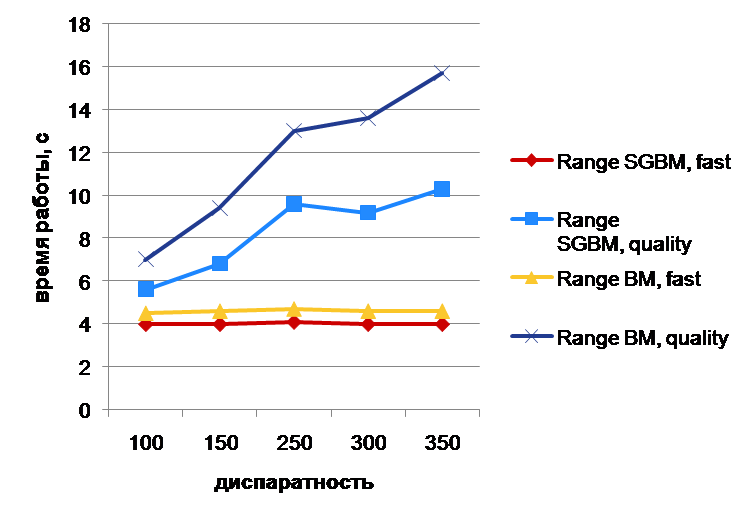
\includegraphics[scale=1]{7.png}}
\caption{Сравнение подходов подсчёта попиксельных стоимостей.}
\label{3}
\end{figure}

В табл.~\ref{1} указано время работы алгоритма на одном и том же изображении при различных типах подсчёта стоимостей, где $Simple$ - полный подсчёт всех диспаратностей перед основной частью алгоритма, $range$ - подсчёт только допустимых диспаратностей на основе приближенной карты глубины, "runtime" - подсчёт стоимости в случае потребности алгоритма. Замер производился с помощью модифицированного подхода на основе алгоритма BM. 

В ходе второго эксперимента были рассмотрены подходы задания интервала диспаратностей: $fast$ - интервал строится на основе соседнего пикселя, если мы не доверяем текущему и $quality$ - рассматривается весь интервал от $0$ до $max\_disparity$. Результат эксперимента~\ref{2} подтвердил, что подход $fast$ позволяет решать задачу построения карты глубины ассимптотически независимо от максимальной диспаратности. Также мы видим, что при подходе $quality$  имеет значение алгоритм, используемый в качестве приближения. Модифицированный метод, основанный BM, работает по времени пропорционально диспаратности, потому что у алгоритма BM существует множество точек, для которых не найдено сопоставление. График~\ref{3} иллюстрирует данные выводы.


\begin{table}[h!]
   \caption{Зависимость времени выполнения алгоритма от способа задания интервала диспаратностей.}
    \label{2}
    \begin{tabular}{ | l | l | l | p{5cm} |}
    \hline
    Алгоритм & Тип задания интервала &  Диспаратность & Время работы, с \\ \hline
   
SGBM	& FAST	& 100	& 4.0	\\ \hline
SGBM	& FAST	& 150	& 4.0	\\ \hline
SGBM	& FAST	& 250	& 4.1	\\ \hline
SGBM	& FAST	& 300	& 4.0	\\ \hline
SGBM	& FAST	& 350	& 4.0	\\ \hline
SGBM	& QUALITY	& 100	& 5.6	\\ \hline
SGBM	& QUALITY	& 150	& 6.8	\\ \hline
SGBM	& QUALITY	& 250	& 9.6	\\ \hline
SGBM	& QUALITY	& 300	& 9.2	\\ \hline
SGBM	& QUALITY	& 350	& 10.3\\ \hline	
BM		& FAST	& 100	& 4.5	\\ \hline
BM		& FAST	& 150	& 4.6	\\ \hline
BM		& FAST	& 250	& 4.7	\\ \hline
BM		& FAST	& 300	& 4.6	\\ \hline
BM		& FAST	& 350	& 4.6	\\ \hline
BM		& QUALITY	& 100	& 7.0	\\ \hline
BM		& QUALITY	& 150	& 9.4	\\ \hline
BM		& QUALITY	& 250	& 13.0\\ \hline
BM		& QUALITY	& 300	& 13.6\\ \hline
BM		& QUALITY	& 350	& 15.7\\ 
    \hline
    \end{tabular}
\end{table}

В табл.~\ref{4} представлено общее сравнение алгоритмов, а также их результаты в системе тестирования алгоритмов стереозрения~\cite{middlebury}. Из таблицы следует, что при использовании модифицированного подхода мы получаем результаты по качеству почти равные с лидером - SGM. В тоже время модифицированный алгоритм на основе BM работает в 4 раза быстрее при потери в качестве 28\%, используя $fast$, и в два раза быстрее при потере в качестве 2.8\%. Таким образом нам выгодно заменить стандартный алгоритм Semi-Global Matching на модифицированный метод на основе BM. 
\begin{table}[h!]
   \caption{Итоговое сравнение различных алгоритмов.}
    \label{4}
    \begin{tabular}{ | l | l | l | p{5cm} |}
    \hline
    Алгоритм & Время работы, с & Процент ошибок \\ \hline
     SGM & 17.4 & 10.9  \\ \hline
    SGBM & 3.8 & 11.9  \\ \hline
    BM & 0.4 &  26.2 \\ \hline
    Range by SGBM, FAST& 4.0 & 11   \\ \hline
    Range by SGBM, QUALITY & 6.7 & 11  \\ \hline
    Range by BM, FAST & 4.0 & 14.4  \\ \hline
    Range by BM, QUALITY & 8.8 & 11.2  \\ 
    \hline
    \end{tabular}
\end{table}

На рис.~\ref{pic:6},~\ref{pic:7},~\ref{pic:8} приведены примеры построенных карт с помощью различных алгоритмов. Заметим, что реализации SGM и модифицированного алгоритма не использует эвристики. А также, если мы найдем алгоритм, выдающий карту глубин с большим количеством "доверенных" пикселей, время выполнения подхода $quality$ упадет без потери качества.

\begin{figure}[h!]
\center{
\includegraphics[scale=0.7]{teddy_RANGEbyBM.png}}
\caption{Карта глубины с основе пары изображений "teddy" с помощью модифицированного алгоритма на основе BM.}
\label{pic:6}
\end{figure}

\begin{figure}[h!]
\center{
\includegraphics[scale=0.7]{teddy_RANGEbySGBM.png}}
\caption{Карта глубины с основе пары изображений "teddy" с помощью модифицированного алгоритма на основе SGBM.}
\label{pic:7}
\end{figure}

\begin{figure}[h!]
\center{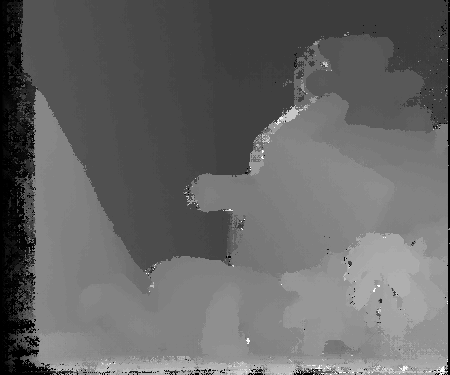
\includegraphics[scale=0.7]{teddy_SGM.png}}
\caption{Карта глубины с основе пары изображений "teddy" с помощью SGM.}
\label{pic:8}
\end{figure}

\clearpage
\startconclusionpage

В работе предложен метод, основанный на алгоритме Semi$-$Global Matching, позволяющий повысить качества карты диспаратности. Метод находит оптимальную конфигурацию глубин карты диспаратности, минимизируя функционал~\ref{minimization}, рассматривая для каждой точки на приближенной карте глубины определенную окрестность возможных глубин.
%TODO не проставился функционал!!

Рассмотрены три метода подсчета попиксельных стоимостей во время алгоритма Semi-Global Matching. 

Проведено сравнение предлагаемого метода со стандартной реализацией SGM, реализацией SGBM и локальным алгоритмом BM. В результате эксперимента получено повышение производительности в два раза при сохранении качества относительно SGM. Повышение качества карт диспаратности получено при использовании карт диспаратности обоих алгоритмов в качестве приближений.





\printbibliography

%\startappendices
%\input{parts/appendix1.tex}

\end{document}
